\section{Backtracking}

\subsection{Descripcion del problema}

	El problema consiste en formar el grupo más grande de agentes comfiables para esto se cuenta con una tabla que representa las encuestas hechas a los agentes. La primera columna de dicha tabla representa el agente encuestado mientras que la segunda columna representa lo que dicho agente informó. Además, cada agente puede elegir informar algo como no, y si lo hace puede hacer tantas declaraciones como desee. Luego la tabla puede ser vacía como tener muchas entradas (notar que la tabla no puede ser infinita). Una vez hechas todas las encuestas se procede a decir cuál es el grupo más grande de agentes confiables. No todo conjunto de agentes es válido por lo que hay ciertas propiedades que tiene que cumplir. La primera es que si un agente dentro del conjunto confía en otro agente, ese agente también debe estar en el grupo, la segunda es que si un agente dentro del conjunto desconfia de otro agente, este no puede ester en el conjunto. Algunos ejemplos serían:
	
\begin{table}[H]
\begin{tabular}{c c}
Agentes & Encuestas  \\ [0.5ex]
\hline
1 & 2 \\
2 & 3 \\
3 & -1 \\
0 & 0 \\ [1ex]
\hline
res: 2 \\
\end{tabular}
\end{table}

\begin{table}[h]
\begin{tabular}{c c}
\centering
Agentes & Encuestas \\ [0.5ex]
\hline
1 & 5 \\
2 & 3 \\
3 & 4 \\
5 & -1 \\ [1ex]
\hline
res: 3 \\
\end{tabular}
\end{table}

\subsection{Solución Propuesta}

	La idea para resolver este problema es considerar todos los posibles casos. Para esto vimos que cada agente puede estar como no en el conjunto, o sea, se va a analizar ambos conjuntos resultantes, uno donde el agente esté en el conjunto y otro donde no esté. A la hora de agregar un agente, llamémoslo i, al conjunto primero vemos que se pueda, esto significa que va a seguir siendo un conjunto válido, para esto vamos a ver un par de cosas. La primera es que nadie en el conjunto desconfíe de i, luego veremos que i no desconfíe de nadie que está en el conjunto, también se verifica que la encuesta del agente tenga sentido lógico, o sea, que no desconfíe de si mismo y, como puede hacer más de una declaración, que no desconfie y confie de un agente. Además para la rama en la cuál no se agrega al agente vereficamos que tenga sentido que no este en el conjunto, esto es que nadie, que este en el conjunto, confie en él. Una vez hecho esto, y  para los otros posibles conjuntos válidos, se elegirá el conjunto con mayor cantidad de agentes. 
	
\subsection{Resolución}
	La técnica de backtracking consiste en pensar conceptualmente en un árbol que contega todas las posibles soluciones. Por esto la solución que propone mi algoritmo es la siguiente:
	
\begin{itemize}
\setlength\itemsep{-0.2em}
\item Partir de la raíz (ningún agente elegido).
\item Comenzar por el primer agente ver si puede ser agregado al conjunto (las consideraciones descriptas en el punto anterior) y considerar que no forme parte del mismo, luego recorrer recursivamente cada una de esas 2 posibilidades para el elemento siguiente (2 ramas).
\item A partir del segundo elemento, recorrer recursivamente cada una de las 2 ramas sólo si ésta es válida, en otras palabras, si puede ser agregado el agente al conjunto. Además si el agente tiene que estar en el conjunto (porque alguien en el conjunto confía en él) la rama que corresponde a no agregar al agente no se recorre ya que no sería una instancia válida del problema.
\item Al llegar a una hoja que esté en el último nivel (cuando la altura del árbol es igual a la cantidad de agentes) se chequea que el conjunto resultante sea válido esto lo hacemos por que a la hora de agregar un agente al conjunto no estamos viendo que si este confia en alguien que no esta en el conjunto se pueda agregar a ese agente en el futuro. Luego si la cantidad de agentes dentro del conjunto resultante es mayor a la que ya tenés, entonces ésta será la mejor solución. Si no, entonces me quedo con la solución que tenía antes.
\end{itemize}
	
\subsection{Pseudocódigo}

\begin{algorithm}[H]
\caption{Backtracking}\label{Ej1}

\begin{algorithmic}[H]
\Procedure{Backtracking}{vector(pair(agente, agente)) encuestas, agentes, ConjAgentes}
\If{Si no me quedan agentes para evaluar}
\If{longitud(ConjAgentes) > solucion}
\State solucion $=$ longitud(ConjAgentes)
\EndIf
\EndIf
\If{PuedoAgregarAgente}
\State Paso Recursivo rama agregueAlAgente
\EndIf
\If{NadieConfiaEnElAgente}
\State Paso Recursivo rama NoAgregoAlAgente
\EndIf
\EndProcedure
\end{algorithmic}
\end{algorithm}

	A la hora de recorrer ambas ramas, se verifica que no genere instancias inválidas. 
\subsection{Demostración de correctitud}

	La técnica descripta anteriormente parte de pensar al problema como un árbol con todas las posibles soluciones. Cada nodo del árbol representa como se va ir modificando nuestro conjunto incluyendo o no a un determinado agente. A pesar de que nuestro algorítmo se basa en esta idea falta decir porque es correcto respecto a nuestro problema. La razón es que recorre las ramas que son válidas según las condiciones del problema y no considera las inválidas. Una vez que tenemos el conjunto de soluciones posibles se queda con la mejor de ellas, en este paso (cuando ya se recorrió todo el árbol) se prodrían considerar las soluciones descartadas pero serían descartas de nuevo ya que no cumplen con lo pedido, lo que hacemos es descartalas antes de llegar al final del árbol para ahorrarnos recorrer dichas ramas. Entonces al final generamos todas las posibles soluciones y nos quedamos con la mejor.

\subsection{Complejidad teórica}
	
	Como dijimos antes la idea conceptual del problema es pensarlo como un árbol de soluciones. Como este árbol contempla todas las posibles soluciones es un árbol completo, ya que por cada nodo tenemos 2 opciones, que forme parte del conjunto o que no forme. Entonces terminamos teniendo un árbol con $2^{i}$ hojas, donde "i" es la cantidad de agentes. Luego para pasar de un nivel del árbol a otro, hacemos O($a^{2}*i$) esto lo pagamos a la hora de ver si el agente es confiable, lo que hacemos es para cada agente recorremos las encuestas ("a") y chequeamos que se pueda agregar al conjunto para esto nos fijamos que las encuestas del agente a agregar no atenten con las encuestas de los agenetes que ya están en el conjunto, además chequeamos que nadie en el conjunto desconfie del agente a agregar. Luego en el último nivel hacemos un chequeo para ver si efectivamente el conjunto es válido, esto se debe a que a la hora de agregar un agente al conjunto no estamos considerando que si este confia en un agente y ese agente no se encuentra en el conjunto lo pueda agregar en el futuro. Para hacer esto tenemos que recorrer una vez mas el conjunto y ver que siga siendo un conjunto válido. Esto nos toma O($i^{2}a$) pasos. Luego, una vez recorrido todo el árbol, terminamos teniendo una complejidad de O($2^{i}*(i*a^{2})*(i^{2}*a)$) = O($2^{i}*i^{3}*a{3}$).
	
\subsection{Experimentación} 

\begin{figure}[h]

\begin{subfigure}{0.5\textwidth}
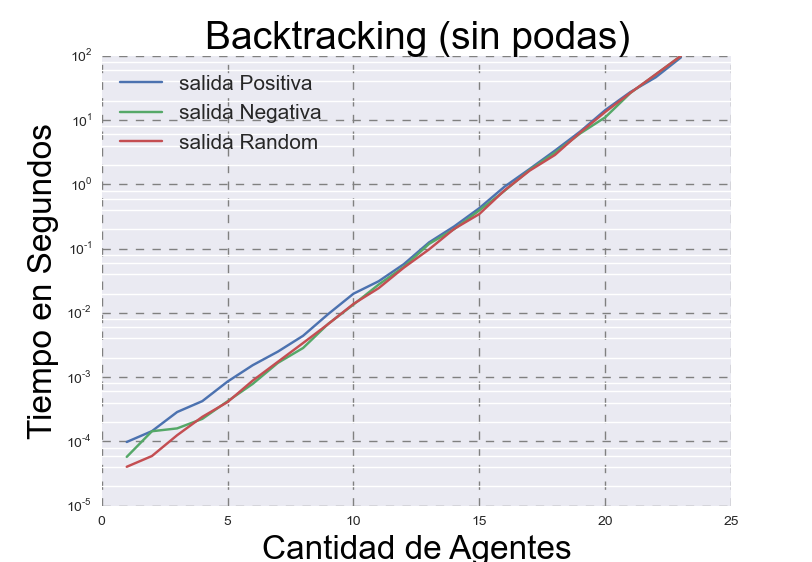
\includegraphics[scale=0.45]{BacktrackingLog.png}
\end{subfigure}
\begin{subfigure}{0.5\textwidth}
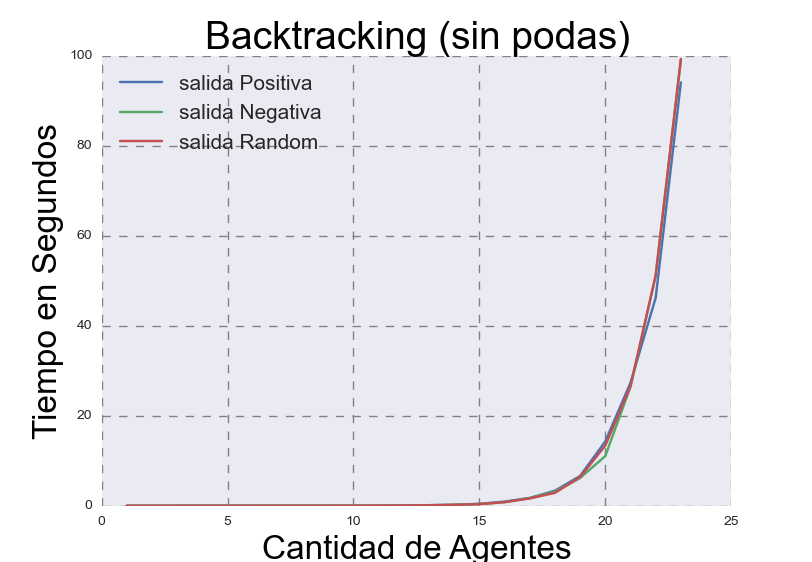
\includegraphics[scale=0.45]{Backtracking.png}
\end{subfigure}

\end{figure}

	En las figuras podemos ver la comparación del algoritmo para diferentes entradas. La muestra fue, para cada uno de los casos 100 muestras de 22 agentes.


